\section{សំណួរ លំហាត់អនុវត្តន៍ និងកិច្ចការផ្ទះ}
\begin{enumerate}
	\item អង្គធាតុមួយមានទម្ងន់ $50\si{\newton}$ ត្រូវបានគេព្យូរដោយប្រើខ្សែទៅនឹងចំណុចនឹងមួយដូចបង្ហាញក្នុងរូប។\\
	ចូរគណនាតំណឹងខ្សែ។
	\begin{figure}[H]
		\centering
		\begin{tikzpicture}[decoration=rope]
			\draw[gray,thin,decorate,rope width=3pt] (2,-.1) to (2,-3);
			\draw[gray!40!black, line width=2.5pt] (-.2,-.3) to (4.2,-.3);
			\fill[left color = white, right color=white, fill opacity=1, top color=gray!40!white, bottom color=gray] (-.2,0) rectangle (4.2,-.3);
			\node[circle,outer color=gray,inner color=white,minimum width=1cm] (radial) at (2,-3) {};
			\node[right] at (2.5,-3) {$50\si{\newton}$};
		\end{tikzpicture}
	\end{figure}
	\item គេតម្លើងប្រព័ន្ធមួយដូចបង្ហាញក្នុងរូប។ ប្រសិនបើតំណឹងរបស់ខ្សែដេកស្មើនឹង $30\si{\newton}$។\\
	ចូររកទម្ងន់របស់អង្គធាតុដែលគេយកទៅព្យូរ។
	\begin{figure}[H]
		\centering
		\begin{tikzpicture}[decoration=rope]
			\coordinate (O) at (0,0);
			\coordinate (A) at (.5,-.1);
			\coordinate (B) at (2,-2);
			\coordinate (C) at (2,0);
			\draw[dashed] (B) to (C);
			\pic [draw, ->, "$50^\circ$", angle eccentricity=1.5, angle radius=1cm] {angle = C--B--A};
			\draw[gray,thin,decorate,rope width=3pt] (A) to (B);
			\draw[gray,thin,decorate,rope width=3pt] (B) to (5.7,-2);
			\draw[gray,thin,decorate,rope width=3pt] (2,-1.9) to (2,-3);
			\fill[left color = white, right color=white, fill opacity=1, top color=gray!40!white, bottom color=gray] (O) rectangle (6,-.3);
			\fill[right color=gray!40!white, left color=gray] (5.7,-.3) rectangle (6,-3);
			\node[circle,outer color=gray,inner color=white,minimum width=.1cm] (radial) at (B) {};
			\node[circle,outer color=gray,inner color=white,minimum width=1cm] (radial) at (2,-3) {};
			\node[right] at (3,-2.5) {$30\si{\newton}$};
		\end{tikzpicture}
	\end{figure}
	\item គេតម្លើងប្រព័ន្ធមួយដូចបង្ហាញក្នុងរូប។\\
	ចូររកតម្លៃនៃ $T_{1}$ និង $T_{2}$ ប្រសិនបើទម្ងន់របស់អង្គធាតុដែលត្រូវបានគេព្យូរគឺ $600N$។
	\begin{figure}[H]
		\centering
		\begin{tikzpicture}[decoration=rope]
			\coordinate (O) at (0,0);
			\coordinate (A) at (5.5,-.1);
			\coordinate (B) at (4,-2);
			\coordinate (C) at (4,0);
			\coordinate (block) at (4,-3);
			\pic [draw, ->, "$50^\circ$", angle eccentricity=1.5, angle radius=1cm] {angle = O--A--B};
			\draw[gray,thin,decorate,rope width=3pt] (A) to (B);
			\draw[gray,thin,decorate,rope width=3pt] (B) to (.3,-2);
			\draw[gray,thin,decorate,rope width=3pt] (4,-1.9) to (block);
			\fill[left color = white, right color=white, fill opacity=1, top color=gray!40!white, bottom color=gray] (O) rectangle (6,-.3);
			\fill[left color=gray!40!white, right color=gray] (0,-.3) rectangle (.3,-3);
			\node[circle,outer color=gray,inner color=white,minimum width=.1cm] (radial) at (B) {};
			\node[circle,outer color=cadetgrey,inner color=white,minimum width=1cm] (radial) at (block) {};
			\node[below] at (2,-2) {$T_{1}$}; 
			\node[right] at (4.5,-1.5) {$T_{2}$};
			\node[right] at (4.5,-3) {$600\si{\newton}$};
		\end{tikzpicture}
	\end{figure}
	\item គេតម្លើងប្រព័ន្ធមួយដូចបង្ហាញក្នុងរូប។\\ ប្រសិនបើគេដឹងថា តំណឹងរបស់ខ្សែ $T_{1}$ ស្មើនឹង $30N$ ចូររកតំណឹងរបស់ខ្សែ $T_{2}$ និងតម្លៃទម្ងន់របស់វត្ថុ។
	\begin{figure}[H]
		\centering
		\begin{tikzpicture}[decoration=rope]
			\coordinate (O) at (0,0);
			\coordinate (A) at (5.5,-.1);
			\coordinate (B) at (4,-2);
			\coordinate (C) at (4,0);
			\coordinate (D) at (.5,-.2);
			\coordinate (block) at (4,-3);
			\pic [draw, ->, "$60^\circ$", angle eccentricity=1.5, angle radius=1cm] {angle = O--A--B};
			\pic [draw, <-, "$50^\circ$", angle eccentricity=1.5, angle radius=1.2cm] {angle = B--D--A};
			\draw[gray,thin,decorate,rope width=3pt] (A) to (B);
			\draw[gray,thin,decorate,rope width=3pt] (B) to (D);
			\draw[gray,thin,decorate,rope width=3pt] (4,-1.9) to (block);
			\fill[left color = white, right color=white, fill opacity=1, top color=gray!40!white, bottom color=gray] (O) rectangle (6,-.3);
			\node[circle,outer color=gray,inner color=white,minimum width=.1cm] (radial) at (B) {};
			\node[circle,outer color=cadetgrey,inner color=white,minimum width=1cm] (radial) at (block) {};
			\node[below] at (2,-1) {$T_{1}$}; 
			\node[right] at (4.5,-1.5) {$T_{2}$};
		\end{tikzpicture}
	\end{figure}
	\item ប្រអប់មួយមានទម្ងន់ $100\si{\newton}$ ស្ថិតនៅស្ងៀមនៅលើកម្រាលឥដ្ឋ។ ប្រសិនបើគេដឹងថា មេគុណកកិតស្តាទិចរវាងប្រអប់នេះ នឹងកម្រាលឥដ្ឋស្មើនឹង​ $0.4$។\\ ចូររកក​​ម្លាំងអប្បរមា $F$ ដែលត្រូវប្រើលើប្រអប់នេះដើម្បីឲ្យប្រអប់នេះចាប់ផ្តើមធ្វើចលនា(ដូចរូប)។
	\begin{figure}[H]
		\centering
		\begin{tikzpicture}[>=Stealth]
			\coordinate (O) at (0,.1);
			\coordinate (A) at (3.5,.5);
			\coordinate (B) at (5,.5);
			\coordinate (F) at (5,1.5);
			\fill[pattern=bricks, pattern color=black, preaction={fill=lightpink}] (O) rectangle (6,-.3);
			\filldraw[gray!40!black,fill=cadetgrey] (2.5,.1) rectangle (3.5,1);
			\draw[->, line width=2pt] (A)--(F);
			\draw[dashed] (A)--(B);
			\node[right] at (5,1.4) {$\vec{F}$};
			\pic [draw, ->, "$30^\circ$", angle eccentricity=1.5, angle radius=1cm] {angle = B--A--F};
		\end{tikzpicture}
	\end{figure}
	\item ប្រអប់មួយមានទម្ងន់ $50\si{\newton}$ ត្រូវបានគេធ្វើឲ្យវារអិលនៅលើកម្រាលឥដ្ឋដោយល្បឿនថេរ ត្រូវប្រើកម្លាំង $25\si{\newton}$ តាមទិសដូចបង្ហាញក្នុងរូបខាងក្រោម។
	\begin{enumerate}[k,2]
		\item ចូររកកម្លាំងកកិតដែលកើតមានពេលដែលប្រអប់មានចលនា។
		\item រកកម្លាំង​​ផ្គុំកែង។
	\end{enumerate}
	\begin{figure}[H]
		\centering
		\begin{tikzpicture}[>=Stealth]
			\coordinate (O) at (0,.1);
			\coordinate (A) at (3.5,.5);
			\coordinate (B) at (5,.5);
			\coordinate (F) at (5,1.5);
			\fill[pattern=bricks, pattern color=black, preaction={fill=lightpink}] (O) rectangle (6,-.3);
			\filldraw[gray!40!black,fill=cadetgrey] (2.5,.1) rectangle (3.5,1);
			\draw[->, line width=2pt] (A)--(F);
			\draw[dashed] (A)--(B);
			\node[right] at (5,1.4) {$25\si{\newton}$};
			\pic [draw, ->, "$40^\circ$", angle eccentricity=1.5, angle radius=1cm] {angle = B--A--F};
		\end{tikzpicture}
	\end{figure}
	\item ពិនិត្យមើលរូបខាងក្រោម។ អង្គធាតុ $A$ មានម៉ាស $5.0\si{\kilogram}$ អង្គធាតុ $B$ មានម៉ាស $2.0\si{\kilogram}$ ត្រូវបានចងភ្ជាប់គ្នាដោយខ្សែមិនយឺត មិននិងមិនគិតម៉ាសហើយឆ្លងកាត់រ៉កមួយ។ គេឃើញអង្គធាតុ $A$ ផ្លាស់ទីទៅស្តាំឯអង្គធាតុ $B$ ផ្លាស់ទីទៅខាងឆ្វេង។
	ចូរកំណត់សំទុះ និងតំណឹងខ្សែនៃប្រព័ន្ធ។ មេគុណកកិតរវាងអង្គធាតុ $A$ នឹងផ្ទៃតុកឺ $0.2$។
	\begin{figure}[H]
		\centering
		\begin{tikzpicture}[decoration=rope]
			\coordinate (O) at (0,0);
			\node at (O) {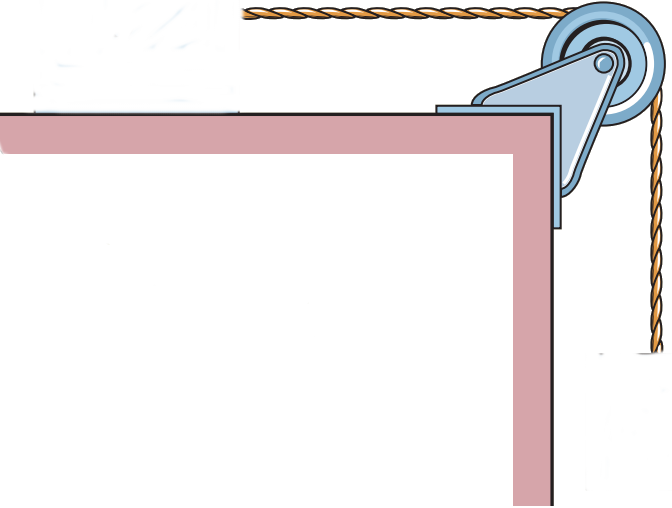
\includegraphics[scale=.22]{pulley_system}};
			\draw[fill=white] (2.5,0) circle (.15cm);
			\draw[fill=white] (0,1.87) circle (.15cm);
			\filldraw[gray!40!black,fill=cadetgrey] (-1.5,1.1) rectangle (0,2.8);
			\filldraw[gray!40!black,fill=cadetgrey] (2,0) rectangle (3,-1);
			\node at (-.7,2) {$A$};
			\node at (2.46,-.5) {$B$};
		\end{tikzpicture}
	\end{figure}
	\item ដុំម៉ាស $A$ ដែលមានម៉ាស $10\si{\kilogram}$ កំពុងរអិលផ្លាស់ទីចុះក្រោមតាមបណ្តោយប្លង់ទេរដែលបង្កើតបានមុំ $30^\circ$ ជាមួយទិសដេក។ មេគុណកកិតស៊ីនេទិចរវាងដុំម៉ាស និងប្លង់ទេរស្មើនឹង $0.5$។ សំទុះទំនាញដី $g=9.80\si{\metre/\second^{2}}$។
	\begin{enumerate}[k,2]
		\item ចូរគូសដ្យាក្រាមកម្លាំងដែលមានអំពើលើដំុំម៉ាស។
		\item រកកម្លាំងប្រតិកម្មកែង។
		\item រកកម្លាំងកកិតដែលមានអំពើលើដុំម៉ាស។
		\item រកសំទុះនៃដុំម៉ាស និងកម្លាំងផ្គួបដែលមានអំពើលើដុំម៉ាស។
	\end{enumerate} 
	\begin{figure}[H]
		\centering
		\begin{tikzpicture}
		\begin{scope}
			\coordinate (A) at (0,2);
			\coordinate (B) at (4,0);
			\coordinate (C) at (0,0);
			\draw (A)--(B)--(C)--cycle;
			\pic [draw, -, "$30^\circ$", angle eccentricity=1.5, angle radius=1cm] {angle = A--B--C};
			\draw[gray!40!black, line width=2.5pt] (-.2,0)--(4.2,0);
			\fill[left color = white, right color=white, fill opacity=1, bottom color=gray!40!white, top color=gray] (-.2,0) rectangle (4.2,-.2);
			\draw[gray!40!black, fill=cadetgrey,rotate around={-26.5:(1,1.75)}] (0,2.18) rectangle (1,1.55);
		\end{scope}
		\end{tikzpicture}
	\end{figure}
	\item គេភ្ជាប់អង្គធាតុពីរដោយខ្សែដែលឆ្លងកាត់រ៉កមួយ(កកិតរវាងខ្សែ និងរ៉កអាចចោលបាន) ដូចរូប រួចគេលែងវត្ថុទាំងនោះដោយល្បឿនដើមស្មើសូន្យ។ គេឲ្យ $m_{1}=2.0\si{\kilogram},~m_{2}=5.0\si{\kilogram}$ និង $\theta=60^{\circ}$។ គេយក $g=9.80\si{\metre/\second^{2}}$។
	\begin{enumerate}[k,2]
		\item គណនាសំទុះនៃអង្គធាតុ។
		\item គណនាតំណឹងខ្សែដែលចង់ភ្ជាប់អង្គធាតុទាំងពីរ។
		\item គណនាល្បឿនរបស់អង្គធាតុនីមួយៗក្រោយពីចេញដំណើរបានរយៈពេល $2.0\si{\second}$។
	\end{enumerate}
	\begin{figure}[H]
		\centering
		\begin{tikzpicture}
			\begin{scope}
				\coordinate (A) at (0,3.5);
				\coordinate (B) at (4,0);
				\coordinate (C) at (0,0);
				\draw[line width=2pt] (1.8,2.6) to (.17,3.9);
				\draw[line width=2pt] (-.43,2) to (-.43,3.5);
				\fill (A) circle (13pt);
				\fill[white] (A) circle (.3cm);
				\draw[fill=white] (1.8,2.6) circle (.2cm);
				\draw[fill=white] (-.45,2) circle (.2cm);
				\draw[fill=white] (A)--(B)--(C)--cycle;
				\fill[gray] (A) circle (.1cm);
				\pic [draw, -, "$\theta$", angle eccentricity=1.5, angle radius=1cm] {angle = A--B--C};
				\draw[gray!40!black, line width=2.5pt] (-.2,0)--(4.2,0);
				\fill[left color = white, right color=white, fill opacity=1, bottom color=gray!40!white, top color=gray] (-.2,0) rectangle (4.2,-.2);
				\draw[gray!40!black, fill=cadetgrey] (-.1,2) rectangle (-.8,1);
				\draw[gray!40!black, fill=cadetgrey,rotate around={-41:(2.5,1.8)}] (1.5,2.5) rectangle (2.5,1.45);
				\node at (-.43,1.5) {$m_{1}$};
				\node at (2.33,2.3) {$m_{2}$};
			\end{scope}
		\end{tikzpicture}
	\end{figure}
	\item រូបខាងក្រោម មេគុណកកិតស៊ីនេទិចរវាងដុំម៉ាស $A$ នឹងតុស្មើ​ $0.2$។ ដុំម៉ាស $m_{A}=25\si{\kilogram}$ និង $m_{B}=15\si{\kilogram}$។ ម៉ាសខ្សែ ម៉ាសរ៉ក និងកកិតរវាងខ្សែនឹងរ៉កអាចចោលបាន។ សំទុះទំនាញដី $g=9.80\si{\metre/\second^{2}}$​\\
	តើអង្គធាតុ $B$ ធ្លាក់បានចម្ងាយប៉ុន្មាន ក្នុងរយៈពេល $3s$ បន្ទាប់ពីគេលែងប្រព័ន្ធ?
	\begin{figure}[H]
		\centering
		\begin{tikzpicture}[decoration=rope]
			\coordinate (O) at (0,0);
			\node at (O) {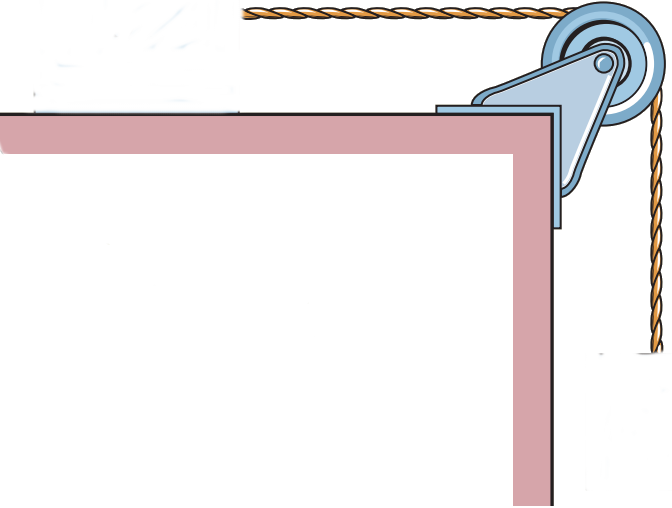
\includegraphics[scale=.18]{pulley_system}};
			\draw[fill=white] (0,1.5) circle (.15cm);
			\filldraw[gray!40!black,fill=cadetgrey] (-1.5,.9) rectangle (0,2.2);
			\node at (-.7,1.5) {$A$};
			\draw[fill=white] (2.05,0) circle (.15cm);
			\filldraw[gray!40!black,fill=cadetgrey] (1.6,-1) rectangle (2.5,0);
			\node at (2.05,-.5) {$B$};
			\draw[>=Stealth, ->, line width=2pt] (2.75, -.5) to (2.75, -1.5) node[right] (3, -1.5) {$\vec{a}$};
			\draw[>=Stealth, ->, line width=2pt] (.5, 1.75) to (1.5, 1.75) node[above] (2, 1.75) {$\vec{a}$};
		\end{tikzpicture}
	\end{figure}
	\item ដុំឈើពីរភ្ជាប់គ្នាដោយខ្សែស្រាលមួយត្រូវបានគេទាញដោយកម្លាំងតាមទិសដេក $\vec{F}$ ដូចរូប។\\ ឧបមា $F=68\si{\newton},~m_{1}=12.0\si{\kilogram}$ និង $m_{2}=18.0\si{\kilogram}$ ហើយកកិតស៊ីនេទិចរវាងដំឈើ នឹងផ្ទៃប៉ះស្មើ $0.100$។
	\begin{enumerate}
		\item ចូរគូសដ្យាក្រាម(វ៉ិចទ័រកម្លាំងលើដុំឈើនីមួយៗ)។
		\item ចូរកំណត់តំណឹងខ្សែ និងសំទុះរបស់ប្រព័ន្ធ។
	\end{enumerate}
	\begin{figure}[H]
		\centering
		\begin{tikzpicture}[>=Stealth, decoration=rope]
			\coordinate (O) at (-1,.1);
			\coordinate (A) at (3.5,.6);
			\coordinate (B) at (5,.6);
			\coordinate (F) at (5,.6);
			\fill[pattern=bricks, pattern color=black, preaction={fill=lightpink}] (O) rectangle (6,-.3);
			\draw[gray,thin,decorate,rope width=3pt] (.3,.55) to (2.5,.6);
			\filldraw[gray!40!black,fill=cadetgrey] (-.5,.1) rectangle (.5,1);
			\filldraw[gray!40!black,fill=cadetgrey] (2.5,.1) rectangle (3.5,1.2);
			\draw[->, line width=2pt] (A)--(F);
			\draw[dashed] (A)--(B);
			\node[above] at (5,.6) {$F$};
			\node at (0,.6) {$m_{1}$};
			\node at (3,.6) {$m_{2}$};
			\node[above] at (1.5,.6) {$T$};
		\end{tikzpicture}
	\end{figure}
	\item នៅអាកាសយានដ្ឋានមួយ ស្រ្តីម្នាក់កំពុងទាញវ៉ាលីរបស់គាត់ដែលមានម៉ាស $20.0\si{\kilogram}$ ឲ្យផ្លាស់ទីដោយល្បឿនថេរ ហើយប្រើកម្លាំងដែលមានទិសដៅបង្កើតបានមុំ $\theta$ ជាមួយអ័ក្សដេក និងមានតម្លៃ $35.0\si{\newton}$ ដូចបង្ហាញក្នុងរូប។\\ កម្លាំងកកិតដែលមានអំពើលើវ៉ាលីមានតម្លៃស្មើ $20.0\si{\newton}$។
		\begin{enumerate}
			\item ចូរគូសដ្យាក្រាមកម្លាំងដែលមានអំពើលើវ៉ាលីនេះ។
			\item រកតម្លៃរបស់មុំ $\theta$។
			\item រកតម្លៃរបស់កម្លាំងកែងដែលផ្ទៃដីមានអំពើលើវ៉ាលី។
	\end{enumerate}
	\begin{figure}[H]
		\centering
		\begin{tikzpicture}
			\coordinate (A) at (-.5,-1);
			\coordinate (B) at (.5,0);
			\coordinate (C) at (.5,-1);
			\draw [line width=2pt](A) to (B);
			\draw [dashed](A) to (C);
			\node at (0,0) {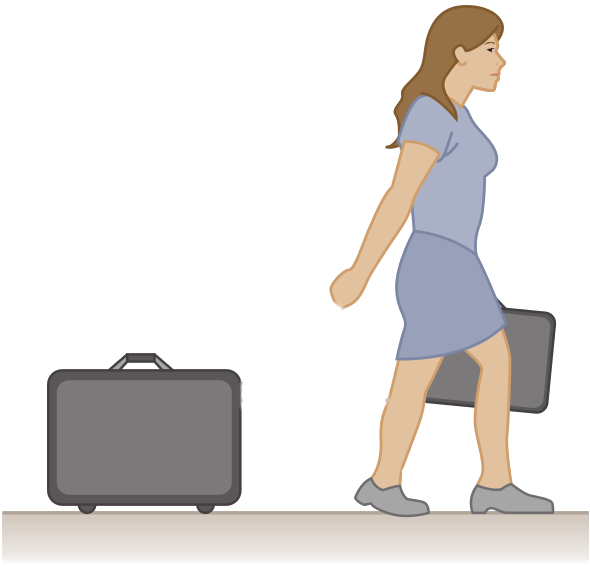
\includegraphics[scale=.25]{woman}};
			\pic [draw, -, "$\theta$", angle eccentricity=1.5, angle radius=.5cm] {angle = C--A--B};
		\end{tikzpicture}
	\end{figure}
	\item គេចោលអង្គធាតុមួយពីក្រោមឡើងទៅលើតាមទិសឈរដោយល្បឿនដើម $30\si{\metre/\second}$។\\ ក្រោយរយៈពេល $2.5\si{\second}$ អង្គធាតុឡើងដល់ចំណុចខ្ពស់បំផុត។\\ គណនាកម្លាំងទប់មធ្យមនៃខ្យល់ដែលរងដោយអង្គធាតុក្នុងពេលវាឡើង។ គេឲ្យម៉ាសអង្គធាតុ $40\si{\gram}$ និង $g=9.80\si{\metre/\second}$។
	\item តើគេត្រូវការកម្លាំង​ហ្រ្វាំងប៉ុន្មានញូតុន ដើម្បីបញ្ឈប់រថយន្តមួយមានម៉ាស $1500\si{\kilogram}$ ដែលកំពុងបើកបរដោយល្បឿន $100\si{\kilo\metre/\hour}$ ឲ្យនៅស្ងៀមក្នុងចម្ងាយ $55\si{\metre}$។
\end{enumerate}